\section{Volumen und Oberflächenrechnung}
	\subsection{Volumen eines beschränkten Körpers}
	Das Volumen eines beschränkten Körpers $K \subset \R^n$ erhalten wir als das Gebietsintegral 
	\begin{equation}
		V(K) = \int_K 1 d\vec{x}
	\end{equation}
	falls das obige Integral existiert.
	
	\subsection{Prinzip von Cavalieri (1598-1647)}
	Sind 2 Körper und eine Gerade im $\R^n$ gegeben und sind die Inhalte der 2 Schnitte der Körper mit jeder ($n-1$) dimensionalen Ebene senkrecht zur Geraden gleich, so haben die Körper auch dasselbe Volumen. 
	\begin{bsp}
	Halbkugel und Zylinder: \newline
	  \begin{figure}[H] 
		  \centering
		  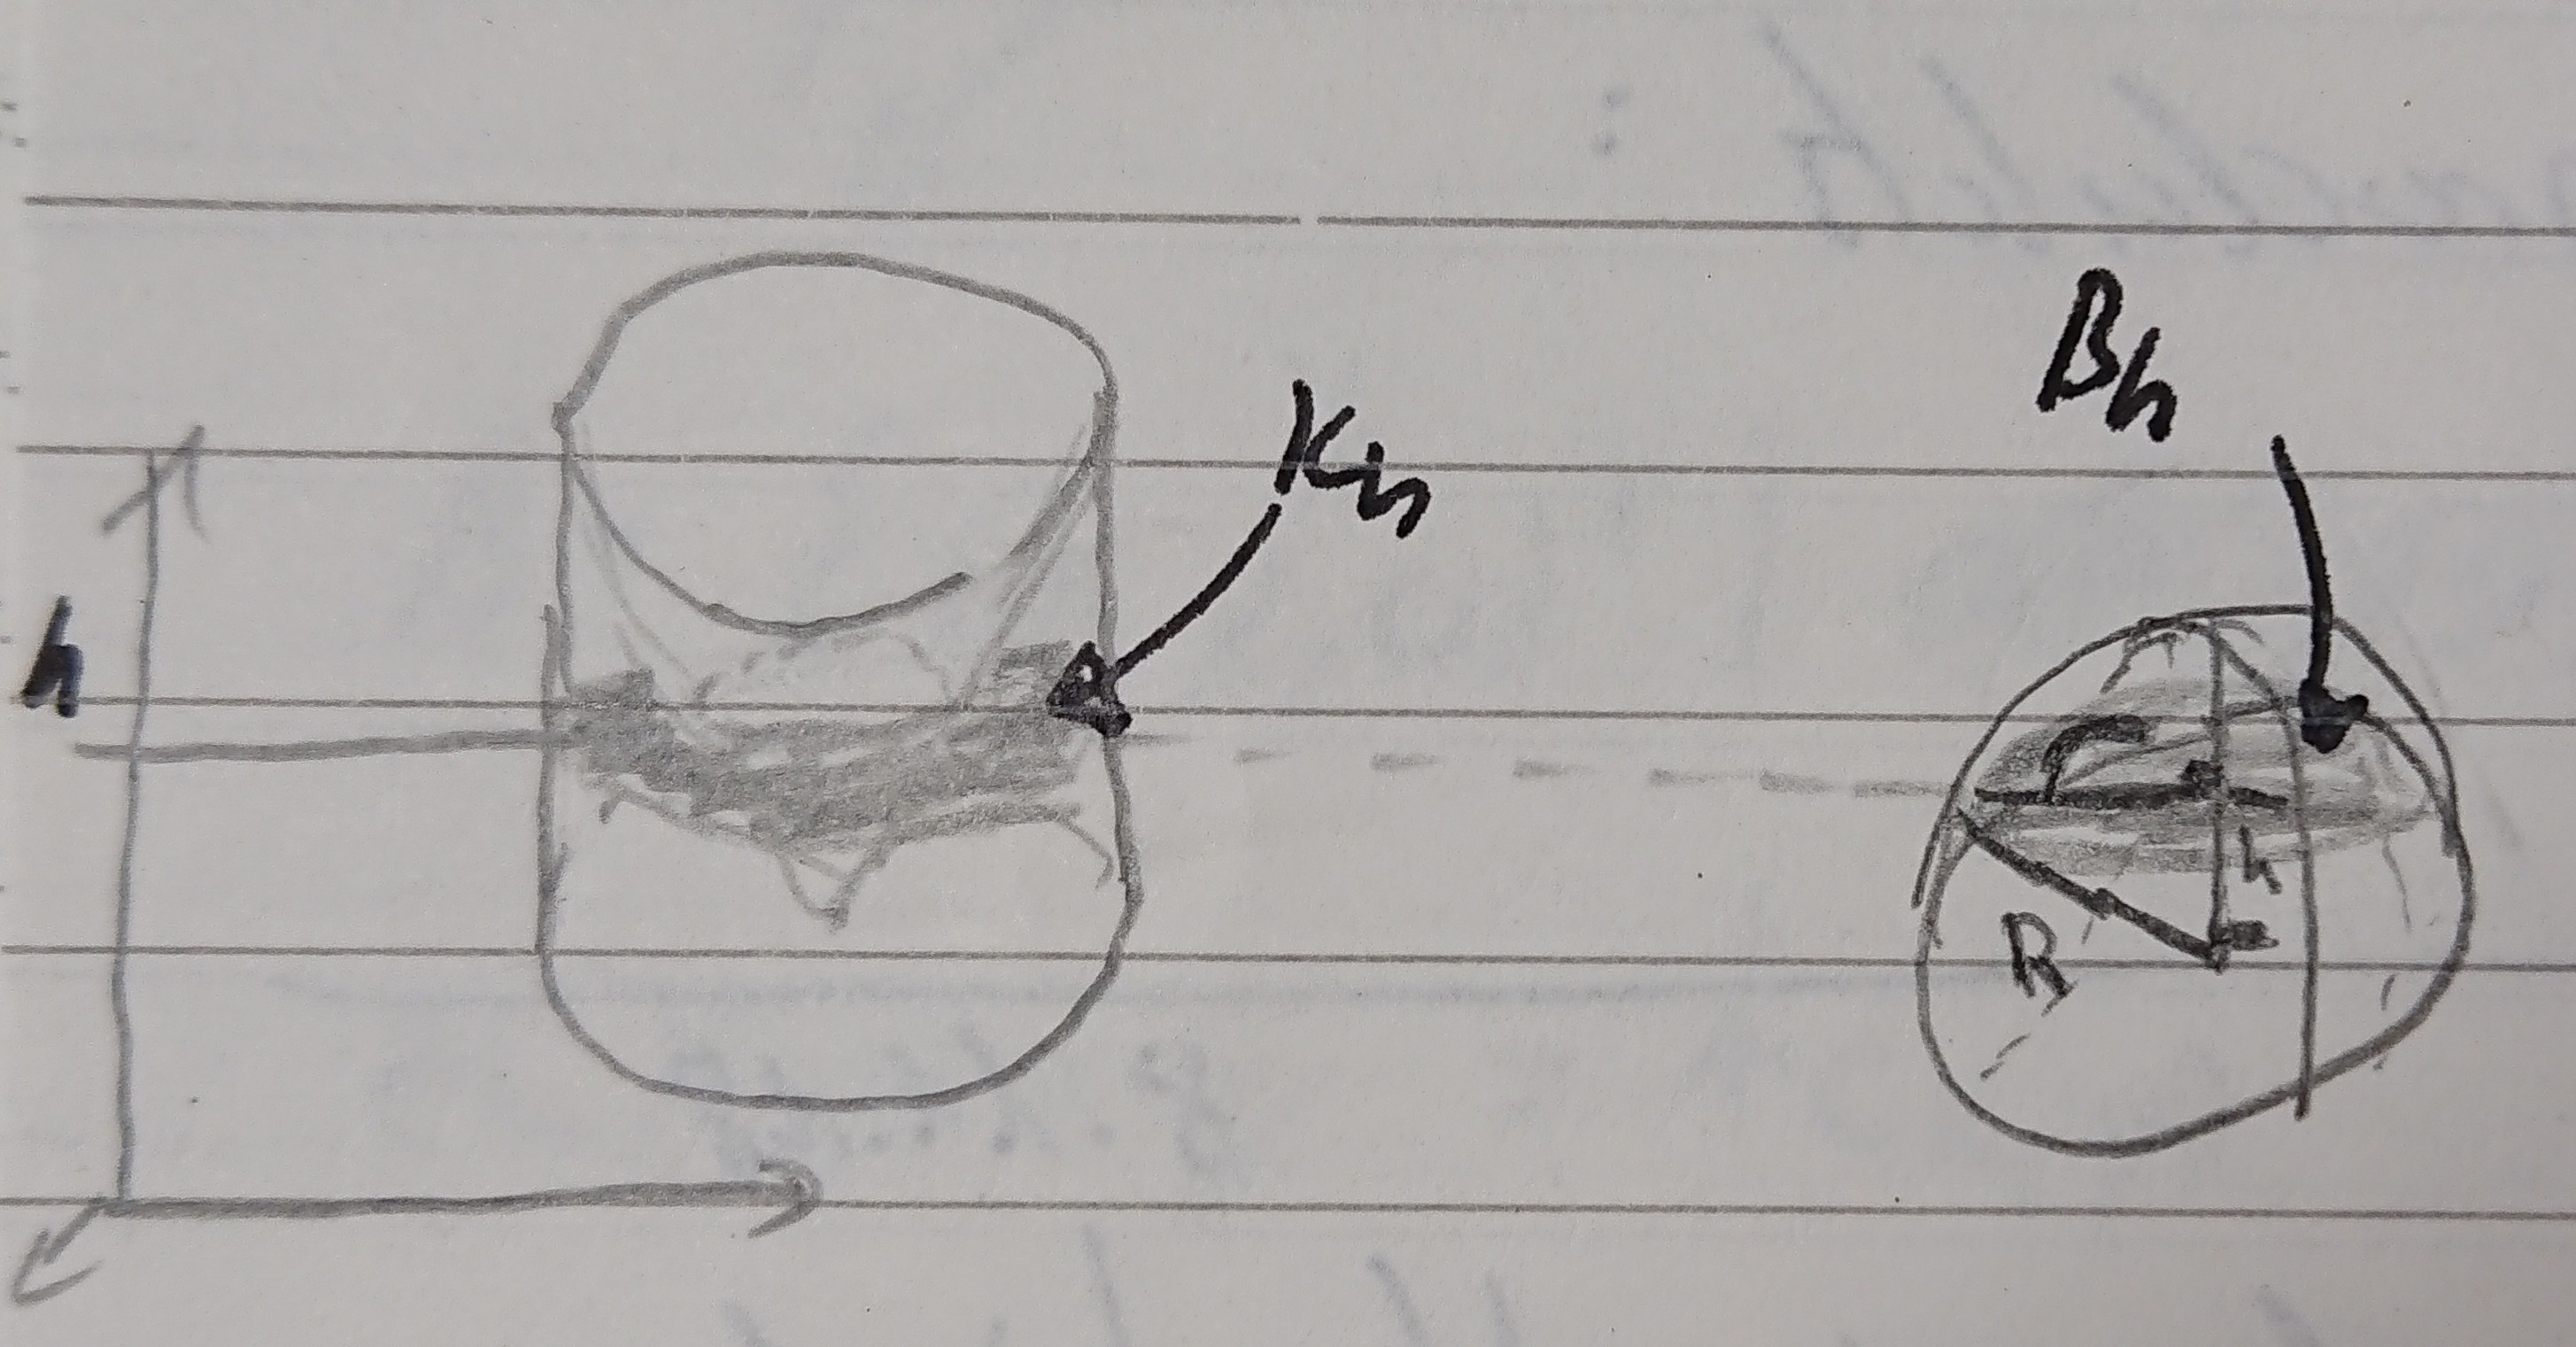
\includegraphics[width=0.5\textwidth]{./img/vol_cavalieri.jpg}
		  \caption{Cavalieri Beispiel}
		  \label{fig:vol_caval}
	  \end{figure}
	  \vspace{-0.5cm}
	Das Volumen der Halbkugel stimmt mit dem Zylinder mit heraus geschnittenem Kegel überein, wenn beide Körper denselben Kreis als Grundfläche haben.\newline \newline
	Aus Vorlesung der Vollständigkeit halber: Nach Fubini gilt für $E subset \R^n \times \R^m$
	\begin{align}
		V_{n+m}(E) &= \int_E \;d(x,y) \; 1 = \int_{\R^n} \dx \int_{E \times\R^m} \dy \;1 \nonumber \\
		&= \int_{\R^n} \dx \; v_m(E_x)
	\end{align}
	Insbesondere im $\R^3$
	\begin{equation}
		v_3(E) = \int_\R \dz \;v_2(E_2)
	\end{equation}
	Nun zu vorangegangenem Beispiel: \newline
	Die Halbkugel sei gegeben durch: Radius = $R$, Schnittfläche auf Höhe $h$ = $B_h$. Dann gilt:
	\begin{equation*}
		v(B_h) = \pi r^2 = \pi(R^2 - h^2) \qquad, r^2 = R^2 - h^2
	\end{equation*}
	Wobei $B_h \in \R^2$ also einen Flächeninhalt darstellt.\newline
	Der Zylinder sei gegeben durch: Radius = $R$, Höhe $h = R$, Schnittfläche auf höhe $h = K_h$. Dann gilt:
	\begin{equation*}
		v(K_h) = R^2 \pi - h^2 \pi = \pi(R^2 - h^2) = v(B_h)
	\end{equation*}
	Also ergibt sich das Volumen im $\R^3$ nach Cavalieri zu
	\begin{align*}
		v(B) = v(K) = \underbrace{R^3  \pi}_{Vol. Zyl.} - \underbrace{R^2 \frac{1}{3} \pi h}_{Vol. Kegel} &\overset{h = R}{=} R^3 \pi - R^3 \pi \frac{1}{3}\\
		&\;\;=\frac{2}{3}\pi R^3
	\end{align*}
	Somit folgt durch Addition zweier identischer Halbkugeln das Volumen einer Kugel mit Radius $R$, dass mit $\frac{4}{3} \pi R^3$ gegeben ist. Mit dem hier genannten Satz wurden in der Vergangenheit die Volumina vieler einfacher Körper bestimmt.
	\end{bsp}
	
	\subsection{Ablauf der Volumenintegration}
	Der allgemeine Ablauf einer Volumenintegration über einen Nicht-Normalbereich soll im folgenden anhand eines Beispiels gezeigt werden.
	\begin{flalign*}
    	&\text{Angaben zum Beispiel}&
  	\end{flalign*}
  	Das Problem lässt sich wie  in Abbildung \ref{fig:vol_int_bsp_a} in karthesischen Koordinaten beschreiben.
  	\begin{figure}[H] 
		  \centering
		  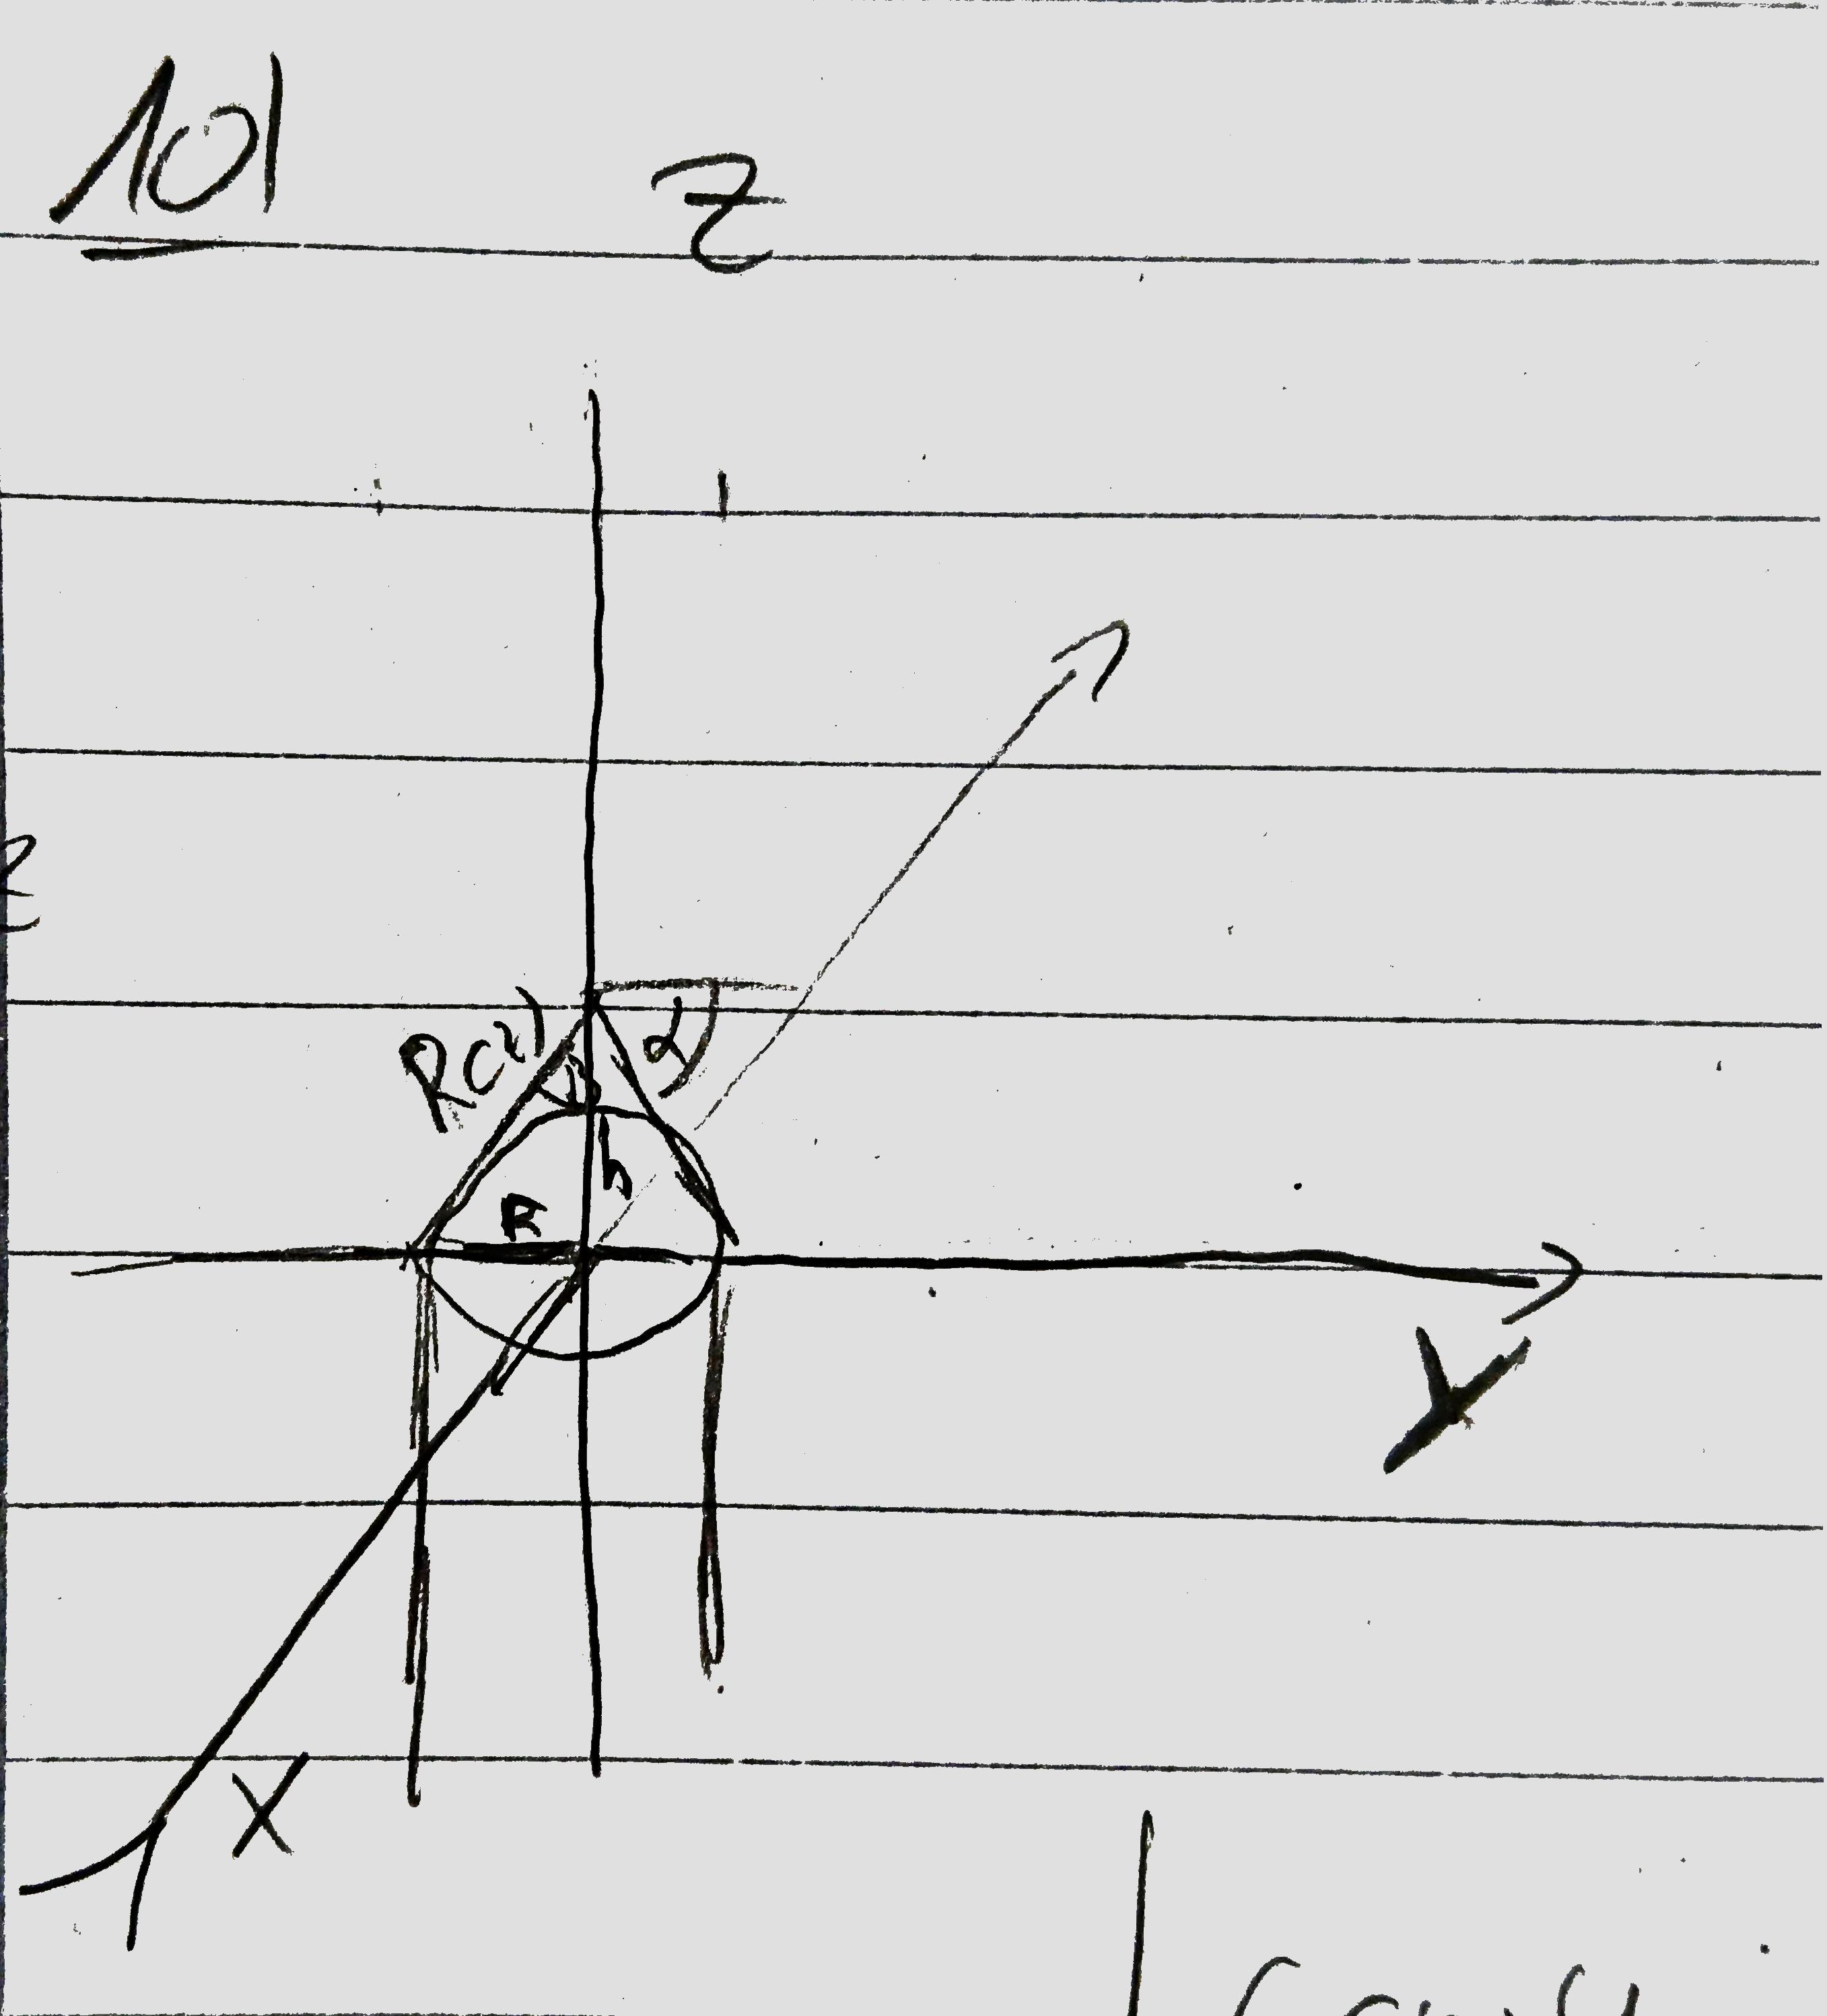
\includegraphics[width=0.3\textwidth]{./img/vol_int_bsp_a.jpg}
		  \caption{Volumenintegral Bsp. Bleistift}
		  \label{fig:vol_int_bsp_a}
	  \end{figure}
	  \vspace{-0.5cm}
	  Ferner ist 
	  \begin{align}
	  	&\alpha = 45^\circ	\Rightarrow \beta = 90^\circ - \alpha = 45^\circ \\
	  	&r = 1 \\
	  	&h = \frac{r}{\tan \beta} = 1 = R
	  \end{align}
	  direkt bekannt oder kann direkt au den Angaben geschlossen werden. Zu bestimmen ist das weggefräste Volumen des in \ref{fig:vol_int_bsp_a} gegebenen Bleistifts.
	\begin{flalign*}
    &\textbf{Schritt 1: } \text{Parametrisierung des zu integrierenden Körpers aufstellen}&
  \end{flalign*}
    \vspace{-0.5cm}
    \begin{align}
    	\gamma &= \vecT{r \cdot \cos \varphi \\ r \cdot \sin \varphi \\ z }\\
    	\text{mit } 0\leq \varphi \leq 2 \pi, \quad &0 \leq z \leq h, \quad 0 \leq r \leq R(z) := R - \frac{R}{h}\cdot z
    \end{align}
      \vspace{-0.5cm}
  \begin{flalign*}
    &\textbf{Schritt 2: } \text{Gegebenenfalls Verzerrungsfaktor bestimmen}&
  \end{flalign*}
    \vspace{-0.5cm}
  \begin{align*}
    \det J_{\gamma} (r,\varphi, z) = \left| 
    \begin{array}{c c c}
    	\cos \varphi & -r\cdot \sin \varphi & 0 \\
    	\sin \varphi & r \cdot \cos \varphi & 0 \\	
    	0 & 0 & 1
    \end{array} \right|
    = r \cos^2\varphi + r \sin^2 \varphi = r
  \end{align*}
    \vspace{-0.5cm}
  \begin{flalign*}
    &\textbf{Schritt 3: } \text{Integral(e) aufstellen}&
  \end{flalign*}
    \vspace{-0.5cm}
  \begin{align*}
  	&\Rightarrow V_{Kegel} = \int_{\gamma} r \;d(\varphi,r,z) = \int_0^{2\pi} \int_0^{R(z)}\int_0^h r \; d\varphi dr dz \\
  	&\Rightarrow V_{Zyl} = \int_{\gamma_z} r \;d(\varphi, r, z) = \int_0^{2\pi} \int_0^R \int_0^h r \;d\varphi dr dz
  \end{align*}
  Wobei zu beachten ist, dass $\gamma_1$ analog zu $\gamma$ parametrisiert ist. Einzig geändert hat sich die obere Schranke für $r$ wie unschwer an den Integralsgrenzen zu erkennen ist.
  \begin{flalign*}
    &\textbf{Schritt 4: } \text{Integral(e) bestimmen}&
  \end{flalign*}	
	 \vspace{-0.5cm}
  \begin{align*}
  	\Rightarrow V_{Kegel} &= \int_0^{2\pi} \int_0^h \frac{1}{2}r^2 \Big|_0^{R(z)} d\varphi dz = \frac{1}{2} \int_0^{2\pi} \int_0^h \left(R - \frac{R}{h}z\right)^2  d\varphi dz \\
  	&= \frac{1}{2} R^2 \int_0^{2\pi} \frac{1}{3} \frac{z^3}{h^2}- \frac{z^2}{h} + z \Big|_0^h  d\varphi = \frac{1}{\cancel{2}}R^2 \left(\frac{h}{3} \cancel{-h+h} \right) \cancel{2}\pi = \frac{1}{3} \pi R^2 h \\
  	\Rightarrow V_{Zyl} &= \int_0^{2\pi} \int_0^h \frac{1}{2}R^2 \; d\varphi dz = \pi R^2 h
  \end{align*}
  \vspace{-0.5cm}
	 \begin{flalign*}
    &\textbf{Schritt 4.1: } \text{Gegebenenfalls Differenz/Summe bilden}&
  \end{flalign*}	
	 \vspace{-0.5cm}
  \begin{align*}
  	\Rightarrow V_{Fr\text{ä}s} = V_{Zyl} - V_{Kegel} = \frac{2}{3} \pi R^2 h \overset{R = h = 1}{=} \frac{2\pi}{3}  
  \end{align*}  
  
	\subsection{Masse und Volumen}
	Idee: Berechnen der Masse als
	\begin{equation*}
		\sum dV  \cdot d\varrho 
	\end{equation*}
	wobei durch $\varrho$ die Dichte des entsprechenden Körpers/Materials gegeben ist. Bildet man nun den Grenzprozess erhält man:
	\begin{equation}
		m(K) = \int_K \varrho(\vec{x}) d\vec{x}
	\end{equation}
	mit $K \subset \R^3$ und $\varrho: K \to \R$.
	Den geometrischen Schwerpunkt erhält man, indem man die Dichte auf $1$ setzt. Es ergibt sich folglich
	\begin{equation}
		\vec{x_{s,geom}} = \frac{1}{A} \int_K \vec{x} \;dA
	\end{equation}
	Idealerweise bestimmt man den Schwerpunkt koordinatenweise.  Im $\R^2$ also beispielsweise:
	\begin{align}
		S &= (s_1,s_2)^T \nonumber \\
		s_1 &= \frac{1}{A} \int_K x \; dA \\
		s_2 &= \frac{1}{A} \int_K y \; dA
	\end{align}
	
	\subsection{Schwerpunkt}
	Eine Wichtige Anwendung der bisher betrachteten Integrale einer Dichte über ein Gebiet anderer Größe ist die Bestimmung des Schwerpunktes. Als Schwerpunkt bezeichnet man jenen Punkt, an dem sich bei fester Ladung alle Drehmomente gegenseitig aufheben. Man sagt Schwerpunkt $\vec{x_s}$ eines Körpers $K$. Bei kontinuierlicher Masseverteilung ergibt sich die Forderung:
	\begin{equation}
		\int_K (\vec{x} - \vec{x_s}) \varrho(\vec{x}) \; d \vec{x} = 0
	\end{equation}
	Damit folgt für die Koordinaten des Schwerpunktes sofort
	\begin{equation}
		\vec{x_s} = \frac{1}{m(K)} \int_K \vec{x} \varrho(\vec{x}) \dX
	\end{equation}